%\vspace{-0.1in}
\section{Introduction}
\label{sec:intro}

In this paper, we present a simple and practical mechanism called \sysname{} to prevent deadlocks
in large deployments of Remote Direct Memory Access (RDMA) over Ethernet (RoCE).

Public cloud providers like Microsoft~\cite{dcqcn} and Google~\cite{timely} are
deploying RoCE in their data centers to provide low latency, high throughput
network transfers with minimal CPU overhead~\cite{dcqcn}.  RoCE uses Priority
Flow Control (PFC) to prevent packet losses due to buffer overflow at the
switches. PFC allows a switch to temporarily pause its immediately upstream
neighbor to prevent buffer overflow. While PFC is effective, it can cause
numerous problems~\cite{dcqcn}, including deadlocks~\cite{rdmaatscale,tcp-bolt,hu2016deadlocks}.

The deadlock problem is not merely theoretical -- our conversations with engineers at large
cloud providers confirm that they have seen the problem in practice and at least
one provider has reported it publicly~\cite{rdmaatscale}. Deadlock is a serious
problem because a deadlock is not transient -- once a deadlock forms, it does not go
away even after the conditions (e.g. a temporary routing loop due to link
failure) that caused its formation have abated~\cite{rdmaatscale}

Deadlock in PFC-enabled network can occur in numerous ways~\cite{hu2016deadlocks},
although in all cases, there is a circular buffer dependency (CBD) among the
group of deadlocked switches. We will describe CBD more formally later in the
paper. For now, the simple example shown in Figure~\ref{fig:deadlock_example} is sufficient --
deadlock is formed, since switch A is blocked by switch B, which is blocked by
C, which is paused by A.

A number of solutions to the deadlock problem are known, and they fall in two
broad categories. The first category consists of solutions that detect the
formation of the deadlock and then use various techniques to break
it~\cite{shpiner2016unlocking}. The problem with these solutions is that they do
not address the root cause of the problem -- and hence cannot guarantee that the
deadlock would not immediately reappear. We do not consider these solutions any
further in this paper. 

The second category of solutions are designed to prevent the key necessary
condition for deadlock formation -- namely, the CBD. There are three ways to
prevent CBD.  Some solutions require centralized, SDN-style routing.  These
solutions are difficult to deploy in existing data centers, without wholesale
infrastructure changes.  The second category of solutions require major changes
to the routing protocols~\cite{xxx}, and thus cannot be implemented using
commodity switches. Many of these solutions also require carefully controlling
path of each packet -- something that is simply not possible with decentralized
routing in presence of link failures~\cite{netpilot}.  Finally, there are
protocols that require creation of numerous priorities and buffer management
according to those priorities. For example, if each of the flows in
Figure~\ref{fig:deadlock_example} had its own priority and was buffered separately at each
switch, there would be no deadlock. However, each
priority class requires reservation of a certain amount of ``headroom'' buffer
space, which limits the total number of priorities one can support. This
headroom depends, among other factors, on the cable length -- since the buffer
must be large enough to absorb all packets in flight.  Given the long cable
lengths used in modern data centers, and the shallow buffers available on
commodify switches, modern data center can typically support only two or three
lossess priorities~\cite{rdmaatscale}.

Given these shortcomings, to the best of our knowledge, no deadlock free routing
solution has been deployed in production networks. 

In contrast, our solution, \sysname{}, can be implemented on existing commodity
switches, and does not require any changes to the existing routing protocol
deployed in the data center. It also does not require an excessive number of
priorities or queues.

The key insight behind \sysname{} is that CBD is caused by flows that take an
``abnormal'' path through the network. For example, a flow may end up on an
``abnormal'' path after BGP reacts to link failure. Not all abnormal paths cause
CBD, however. \sysname{} consists of a clever tagging and buffer management
scheme, such that packets that may cause CBD are automatically detected diverted
to a different queues. When properly configured, this avoids CBD and hence
deadlock. We show that for general topologies, TTL values can be used for
tagging purpose, and we design a greedy algorithm that combines multiple tags
into one lossless priority and effectively reduce the number of required queues.
While the greedy heuristic is not optimal, for popular data center topologies
such as as FatTree, we show that we can reduce the number of priorities even
further by exploiting special structure of the topology.

%% takes the topology and routes that must be lossless as the input, and
%% outputs the buffer configuration and ACL rules that guarantee no deadlock. Our
%% key idea is to tag the packets along the path, and assign each packet to
%% different lossless queues. Without any special assumptions about the topology,
%% TTL is a type of tag that carries implicit information of what path the packet
%% has taken.  Properly configured, we can avoid cyclic buffer dependency using
%% this information.  We 

We have implemented and tested \sysname{} on commodity Arista 7050 Switches that
use the popular Broadcom chipsets.

Our key contributions are as follows: first, using traces from a large cloud
provider's data center, we demonstrate the practical challenges in making RoCE
deadlock-free. We also analyze \sysname{} using simulations and a testbed
implementation. Second, we develop \sysname{} for general topologies and
formally prove that it prevents deadlocks. Third, we optimize \sysname{} for
popular data center topologies such as FatTree to achieve optimal results and
efficiently support multiple application classes.  

\begin{figure}
	\centering
	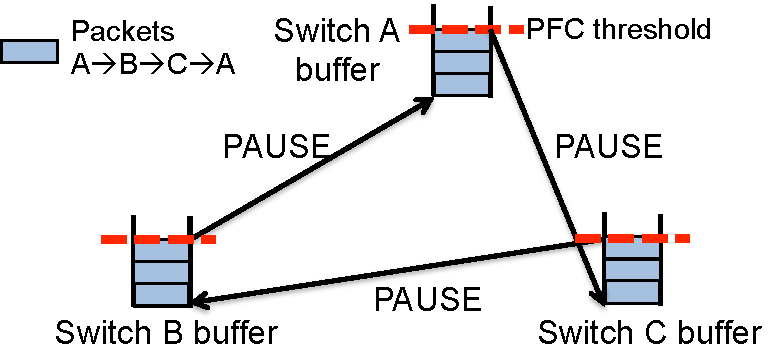
\includegraphics[width=0.3\textwidth] {figs/deadlock}
	\vspace{-0.15in}
	\caption{PFC-induced deadlock: simple illustration}
	\vspace{-0.25in}
	\label{fig:deadlock_example}
\end{figure}
